% Ensure included PDFs (banners) with newer versions embed without warnings
\pdfminorversion=7
\documentclass[aspectratio=169]{beamer}

\makeatletter
% Make LaTeX find theme .sty files in Template
\def\input@path{{../Template/}}
\makeatother
\usepackage{graphicx}
% Make graphics (including banner PDFs) resolvable without TEXINPUTS
\graphicspath{{../Template/}{../Template/banners/}{../../Common_Images/}}

%================================================================%
% Theme and Package Setup
%================================================================%
\usetheme{ucl}
\setbeamercolor{banner}{bg=darkpurple}

% Navigation and Footer
\setbeamertemplate{navigation symbols}{\vspace{-2ex}}
\setbeamertemplate{footline}[author title date]
\setbeamertemplate{slide counter}[framenumber/totalframenumber]

\usepackage[utf8]{inputenc}
\usepackage[british]{babel} % British spelling
\usepackage{amsmath, amssymb, amsthm}
\usepackage{graphicx}
\usepackage{tikz}
\usetikzlibrary{calc, positioning, arrows.meta, shapes.geometric, trees, backgrounds, shapes.misc, graphs, quotes, shadows, fit, patterns} 
\usepackage{pgfplots}
\pgfplotsset{compat=1.17}
\usefonttheme{professionalfonts}
\usepackage{eulervm}
\usepackage{listings}
\usepackage{algorithm}
\usepackage{algpseudocode}
\usepackage{xcolor}
\usepackage{subcaption}

% Define custom colours
\makeatletter
\@ifundefined{color@stone}{%
    \definecolor{stone}{gray}{0.95}%
}{}
\makeatother
\definecolor{darkgreen}{rgb}{0.0, 0.5, 0.0}
\definecolor{uclblue}{cmyk}{1,0.24,0,0.64}
\definecolor{uclred}{cmyk}{0,1,0.62,0}
\definecolor{uclpurple}{cmyk}{0.32,0.42,0,0.55}
\definecolor{uclorange}{cmyk}{0,0.45,0.91,0}

\setbeamercovered{transparent}

% Define theoremblock
\makeatletter
\newenvironment<>{theoremblock}[1]{%
    \begin{block}#2{#1}%
}{\end{block}}
\makeatother

% Section divider slides
\AtBeginSection[]{
  \begin{frame}
    \frametitle{\textbf{\Large\insertsectionhead}}
    \begin{center}
        \huge\textbf{\insertsectionhead}
    \end{center}
  \end{frame}
}

% Maths Macros
\newcommand{\U}{\mathcal{U}}
\newcommand{\V}{\mathcal{V}}
\newcommand{\Z}{\mathcal{Z}}
\newcommand{\R}{\mathbb{R}}
\newcommand{\E}{\mathbb{E}}
\newcommand{\ip}[2]{\langle #1, #2 \rangle}
\newcommand{\norm}[1]{\| #1 \|}
\DeclareMathOperator*{\argmin}{argmin}
\DeclareMathOperator{\prox}{prox}
\DeclareMathOperator{\dom}{dom}
\DeclareMathOperator{\supremum}{sup}
\DeclareMathOperator{\sign}{sign}

\title{Deep Equilibrium Methods (DEQs)}
\subtitle{Part 3: Inverse Problems (DEMs) and Bilevel Learning}
\author[Martin Benning (University College London)]{Martin Benning}
\date[COMP0263]{COMP0263 -- Solving Inverse Problems with Data-Driven Models \\[1cm] 12th March 2026}
\institute[]{University College London}

\begin{document}

% --- Title Frame ---
\begin{frame}
  \titlepage
\end{frame}

% --- Outline ---
\begin{frame}{Lecture Overview}
    \tableofcontents
\end{frame}

\section{Inverse Problems in Imaging (DEMs)}

\begin{frame}{Recap: Inverse Problems in Imaging}
    Recall the definition of a standard linear inverse problem:
    $$ {\color{uclred}f^\delta} = {\color{uclblue}K} {\color{darkgreen}u^\dagger} + e $$
    where ${\color{uclred}f^\delta}$ denotes noisy data, ${\color{uclblue}K}$ the forward operator, ${\color{darkgreen}u^\dagger}$ the true signal and $e$ some noise.
    
    \vspace{1em}
    Standard variational regularisation approximates ${\color{darkgreen}u^\dagger}$ by minimising the energy functional
    
    \begin{theoremblock}{Variational Regularisation}
    $$ u \in \argmin_u \left\{ \frac{1}{2}\|{\color{uclblue}K}u - {\color{uclred}f^\delta}\|_2^2 + \alpha J(u) \right\} $$
    \end{theoremblock}
\end{frame}

\begin{frame}{The Problem with Finite Unrolling}
    Classical deep unrolling applies a finite number $L$ of iterations of an algorithm to solve this problem, giving
    $$ u^{k+1} = f_\theta(u^k; {\color{uclred}f^\delta}), \qquad \hat{u} = u^L $$
    
    \vspace{1em}
    \begin{alertblock}{The Truncation Issue}
        This induces a strong \textbf{train-test coupling}. Increasing the iteration count at inference can create severe out-of-distribution artefacts because the network was optimised strictly for an intermediate iterate $L$, not for true convergence \cite{gilton2021deep}.
    \end{alertblock}
    
    
\end{frame}

\begin{frame}{Deep Equilibrium Models for Imaging (DEMs)}
    Deep Equilibrium Models for imaging (DEMs) overcome this by learning an iteration map whose \textbf{equilibrium} is the reconstruction itself!
    
    \vspace{1em}
    This yields the condition:
    $$ {\color{darkgreen}u^\infty} = f_\theta({\color{darkgreen}u^\infty}; {\color{uclred}f^\delta}) $$
    
    \vspace{1em}
    \begin{itemize}
        \item Makes the architecture effectively \textbf{infinite-depth} with tied weights.
        \item Allows inference to dynamically adapt computation by selecting a stopping tolerance rather than a fixed unrolling depth.
    \end{itemize}
\end{frame}

\begin{frame}{DE-GRAD: Equilibrium Gradient Descent}
    If we consider the classical Gradient Descent update for the energy functional, we obtain
    $$ u^{k+1} = u^k + \eta {\color{uclblue}K^\top}({\color{uclred}f^\delta} - {\color{uclblue}K}u^k) - \eta \alpha \,\nabla J(u^k) $$
    
    \vspace{1em}
    In \textbf{DE-GRAD}, $\nabla J$ is completely replaced by a learned regularisation network $R_\theta$. This yields the equilibrium map
    
    \begin{theoremblock}{DE-GRAD Map \cite{gilton2021deep}}
    $$ f_\theta(u; {\color{uclred}f^\delta}) = u + \eta {\color{uclblue}K^\top}({\color{uclred}f^\delta} - {\color{uclblue}K}u) - \eta R_\theta(u) $$
    \end{theoremblock}
    
    The learned reconstruction is simply the fixed point of this physics-informed gradient-like operator.
\end{frame}

\begin{frame}{DE-PROX: Equilibrium Proximal Gradient Descent}
    Recall the Proximal Gradient Descent iteration for composite objectives:
    $$ u^{k+1} = \operatorname{prox}_{\eta \alpha J}\bigl(u^k + \eta {\color{uclblue}K^\top}({\color{uclred}f^\delta} - {\color{uclblue}K}u^k)\bigr) $$
    
    \vspace{1em}
    \textbf{DE-PROX} replaces the proximal map directly with a trainable denoiser / de-artefacting block $R_\theta$, which gives
    
    \begin{theoremblock}{DE-PROX Map \cite{gilton2021deep}}
    $$ f_\theta(u; {\color{uclred}f^\delta}) = R_\theta\bigl(u + \eta {\color{uclblue}K^\top}({\color{uclred}f^\delta} - {\color{uclblue}K}u)\bigr) $$
    \end{theoremblock}
    
    We reconstruct via the equilibrium condition ${\color{darkgreen}u^\infty} = f_\theta({\color{darkgreen}u^\infty}; {\color{uclred}f^\delta})$.
\end{frame}

\begin{frame}{DE-PROX Architecture Visualised}
    \begin{figure}[htpb]
        \centering
        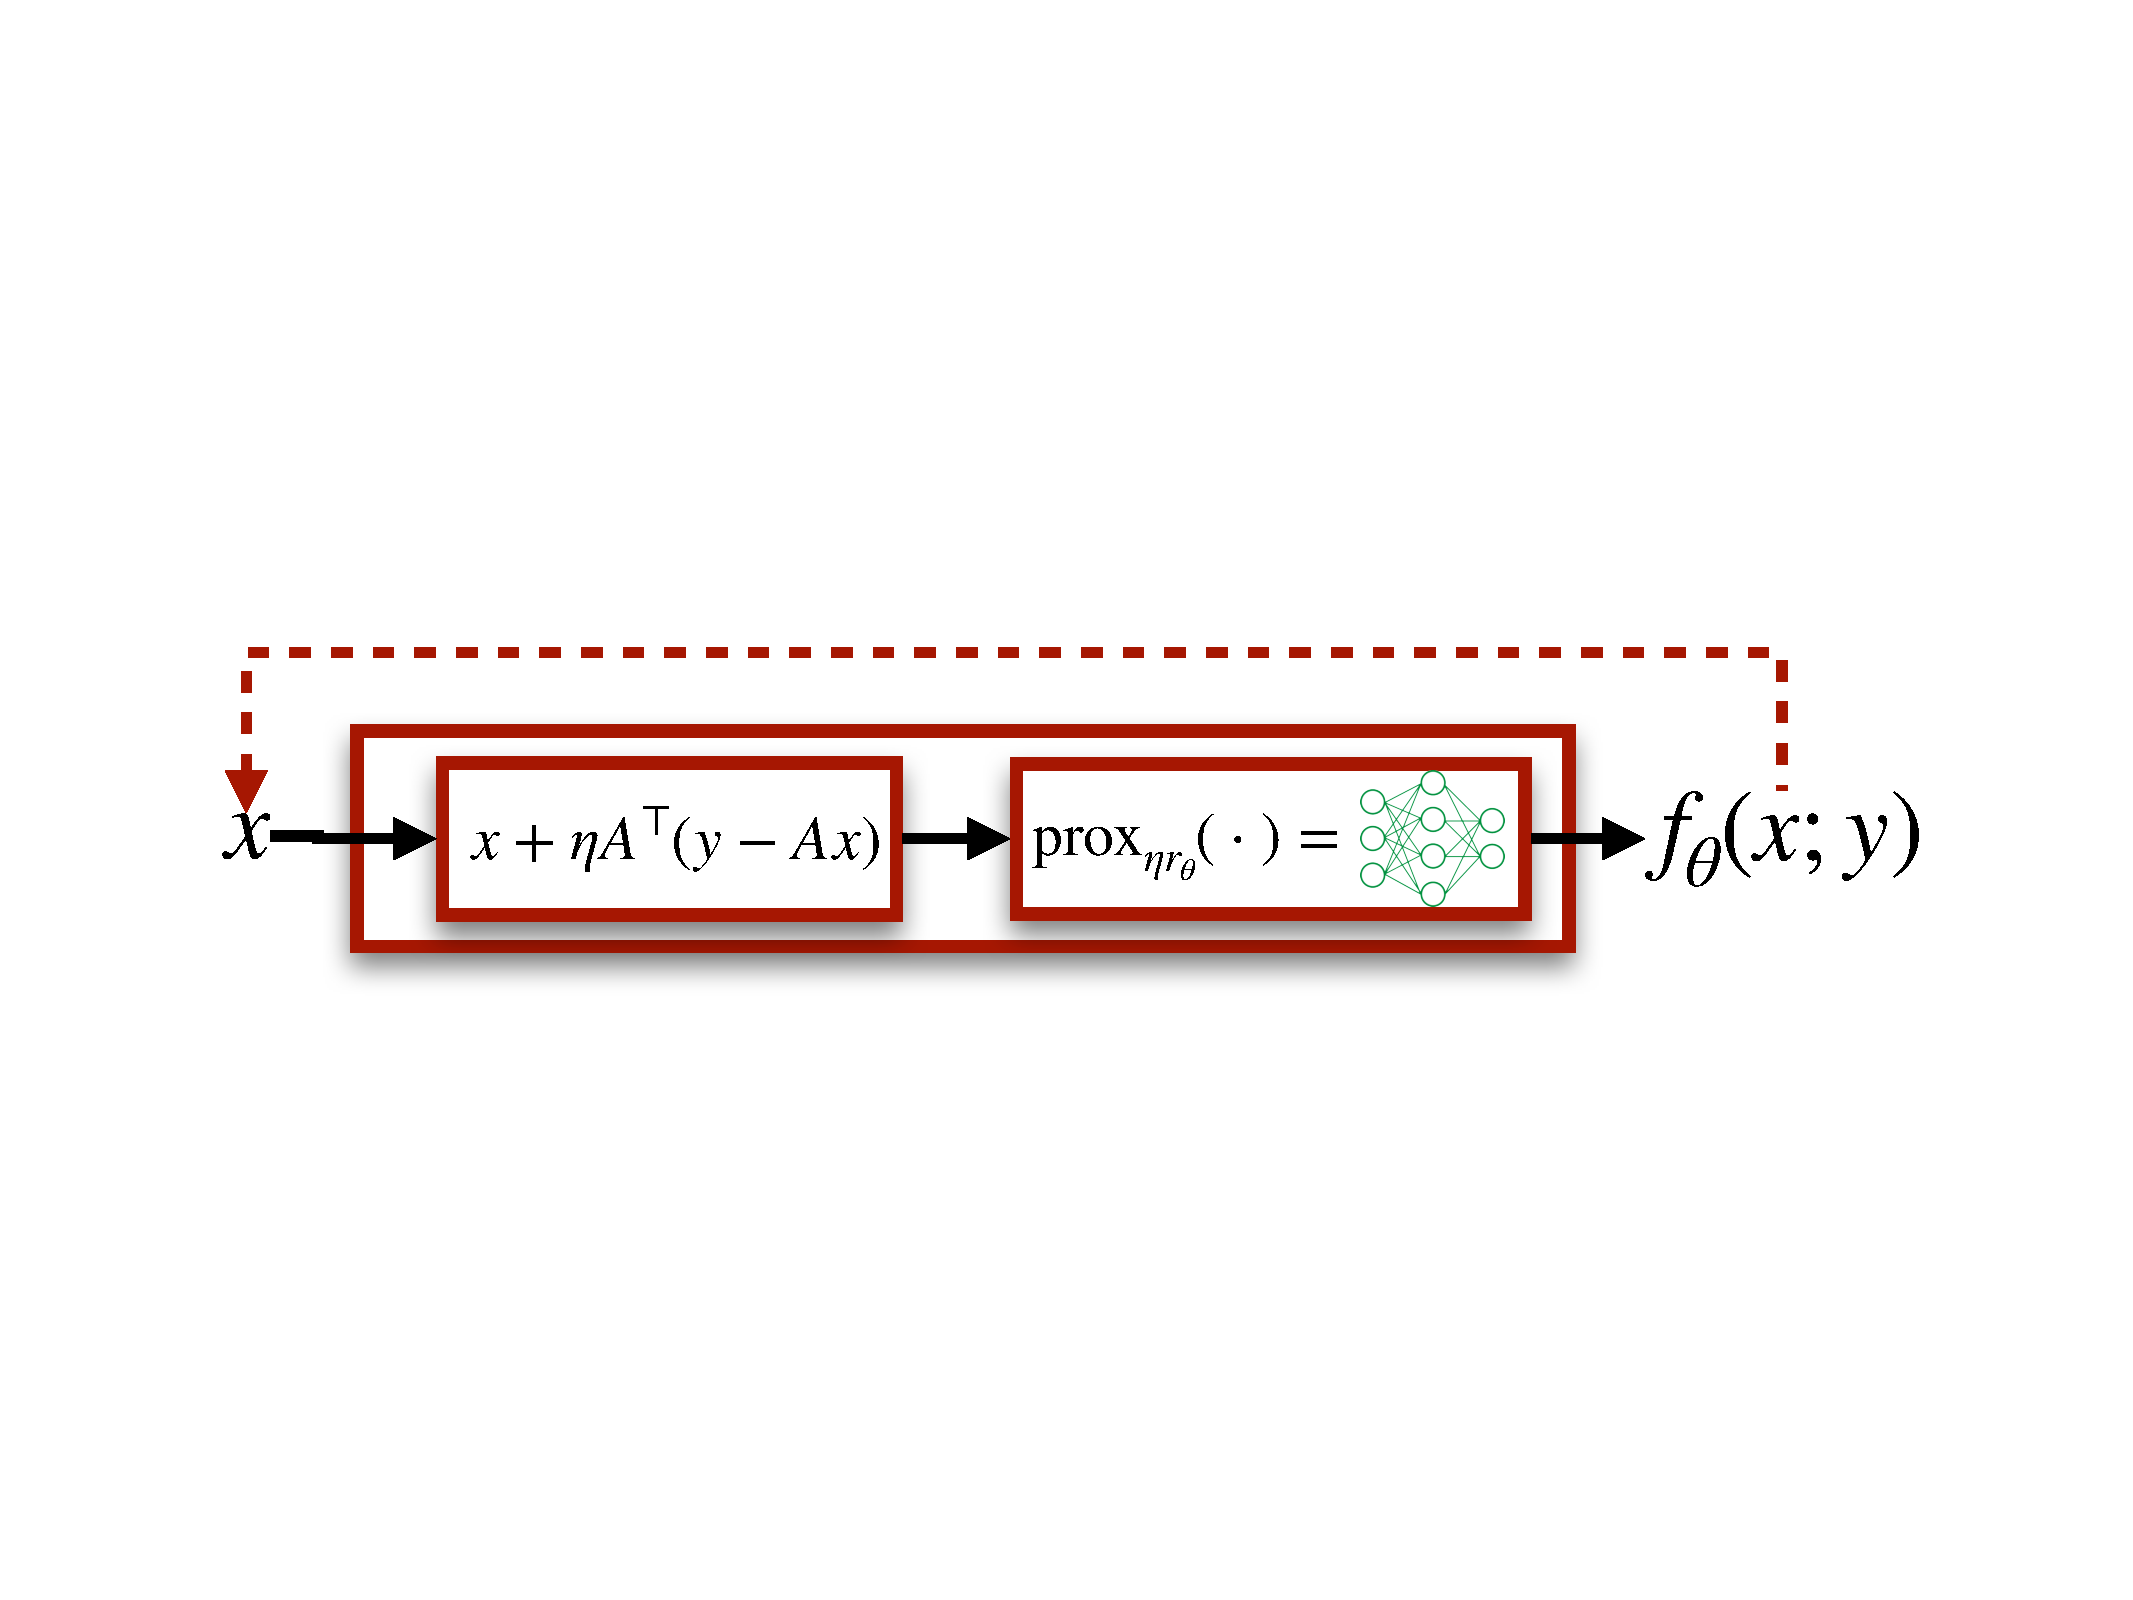
\includegraphics[width=0.7\textwidth]{../Common_Images/deq/DEProx.pdf}
        \caption{Architecture of DE-PROX. The model computes the equilibrium state of an iterative process involving a data-consistency gradient step followed by a learned regularisation block $R_\theta(\cdot)$ \cite{gilton2021deep}.}
        \label{fig:deprox}
    \end{figure}
\end{frame}

\begin{frame}{DE-ADMM: Equilibrium ADMM Splitting}
    Recall the ADMM updates for constrained splitting on the variational problem $z=u$. 
    
    \vspace{1em}
    \textbf{DE-ADMM} replaces $\operatorname{prox}_{\alpha J}$ by $R_\theta$ and interprets the resulting recursion as a fixed-point map on the joint primal-dual state $q = (u,\zeta)$. This yields
    
    $$ q^{k+1} = f_\theta(q^k; {\color{uclred}f^\delta}), \qquad {\color{darkgreen}q^\infty} = f_\theta({\color{darkgreen}q^\infty}; {\color{uclred}f^\delta}) $$
    
    \vspace{1em}
    This elegant formulation preserves the rigorous splitting structure of ADMM while learning the regularisation action entirely end-to-end.
\end{frame}

\begin{frame}{Convergence Guarantees for DEMs}
    How can we mathematically guarantee that these solvers find a fixed point?
    
    \vspace{1em}
    The DEM analysis assumes a \textbf{residual-Lipschitz condition} of the form:
    $$ \|(R_\theta - I)(u) - (R_\theta - I)(u')\| \leq \varepsilon \|u - u'\| $$
    
    \vspace{1em}
    With system parameters defined as $L = \lambda_{\max}(K^\top K)$ and $\mu = \lambda_{\min}(K^\top K)$, we can establish strict contractivity of the induced iteration maps.
\end{frame}

\begin{frame}{Contractivity Bounds}
    \begin{itemize}
        \item \textbf{DE-GRAD} is contractive for step sizes $\eta < 1/(L+1)$, with a Lipschitz factor bounded by $\gamma = 1 - \eta(1+\mu) + \eta\varepsilon$. It converges when $\gamma < 1$.
        \vspace{0.5em}
        \item \textbf{DE-PROX} maintains contractivity when:
        $$ \frac{1}{\mu(1+1/\varepsilon)} < \eta < \frac{2}{L} - \frac{1}{L(1+1/\varepsilon)} $$
        \vspace{0.5em}
        \item \textbf{DE-ADMM} converges under the sufficient condition:
        $$ \alpha > \frac{\varepsilon}{(1+\varepsilon-2\varepsilon^2)\mu} $$
    \end{itemize}
    \vspace{1em}
    These formal results explain why DEM inference can be robustly run to absolute convergence, completely unlike fixed-depth unrolling!
\end{frame}

\begin{frame}{Visual Comparison: 8x Accelerated MRI}
    \begin{figure}[htpb]
        \centering
        \begin{minipage}{0.24\textwidth}
            \centering
            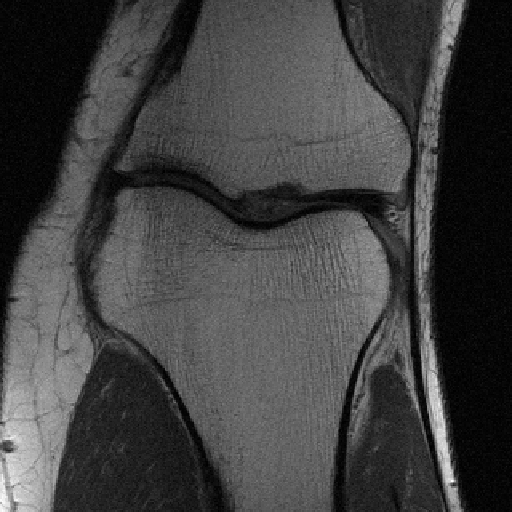
\includegraphics[width=\textwidth]{../Common_Images/deq/groundtruth_mri.png}
            \caption*{Ground truth}
        \end{minipage}
        \hfill
        \begin{minipage}{0.24\textwidth}
            \centering
            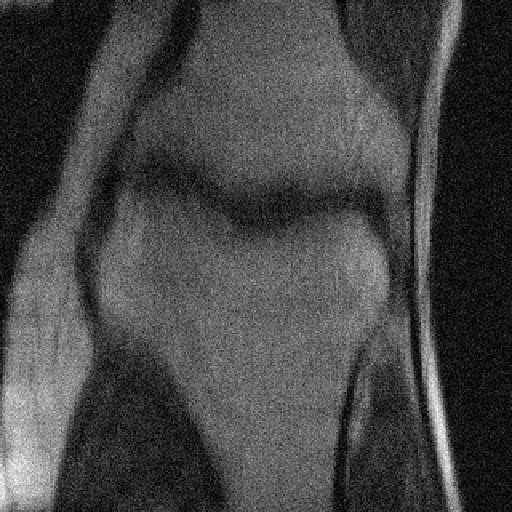
\includegraphics[width=\textwidth]{../Common_Images/deq/ifft_mri_8.png}
            \caption*{IFFT (24.53 dB)}
        \end{minipage}
        \hfill
        \begin{minipage}{0.24\textwidth}
            \centering
            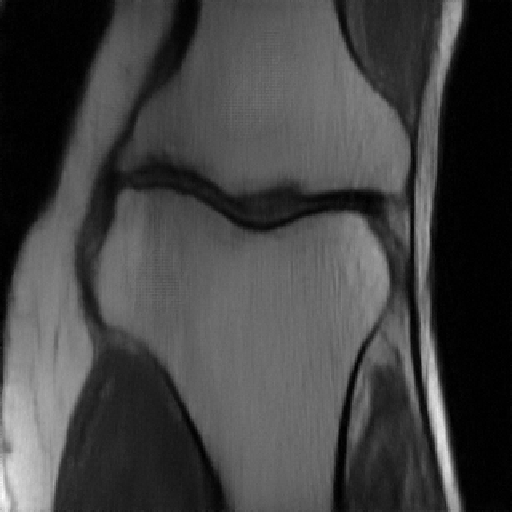
\includegraphics[width=\textwidth]{../Common_Images/deq/duprox_8_31.018515.png}
            \caption*{DU-PROX (31.02 dB)}
        \end{minipage}
        \hfill
        \begin{minipage}{0.24\textwidth}
            \centering
            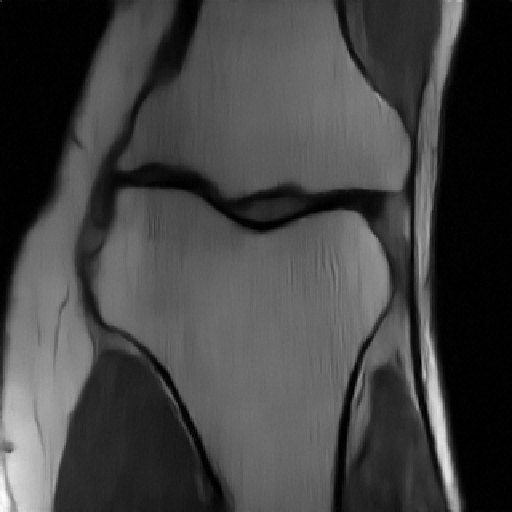
\includegraphics[width=\textwidth]{../Common_Images/deq/deprox_8_32.087868.png}
            \caption*{DE-PROX (32.09 dB)}
        \end{minipage}
        \caption{DE-PROX produces sharper details and achieves higher PSNR compared to finite unrolling (DU-PROX) \cite{gilton2021deep}.}
        \label{fig:mri_reconstruction}
    \end{figure}
\end{frame}

\begin{frame}{Iterations vs. PSNR Analysis}
    \begin{columns}
        \begin{column}{0.5\textwidth}
            \begin{figure}[htpb]
                \centering
                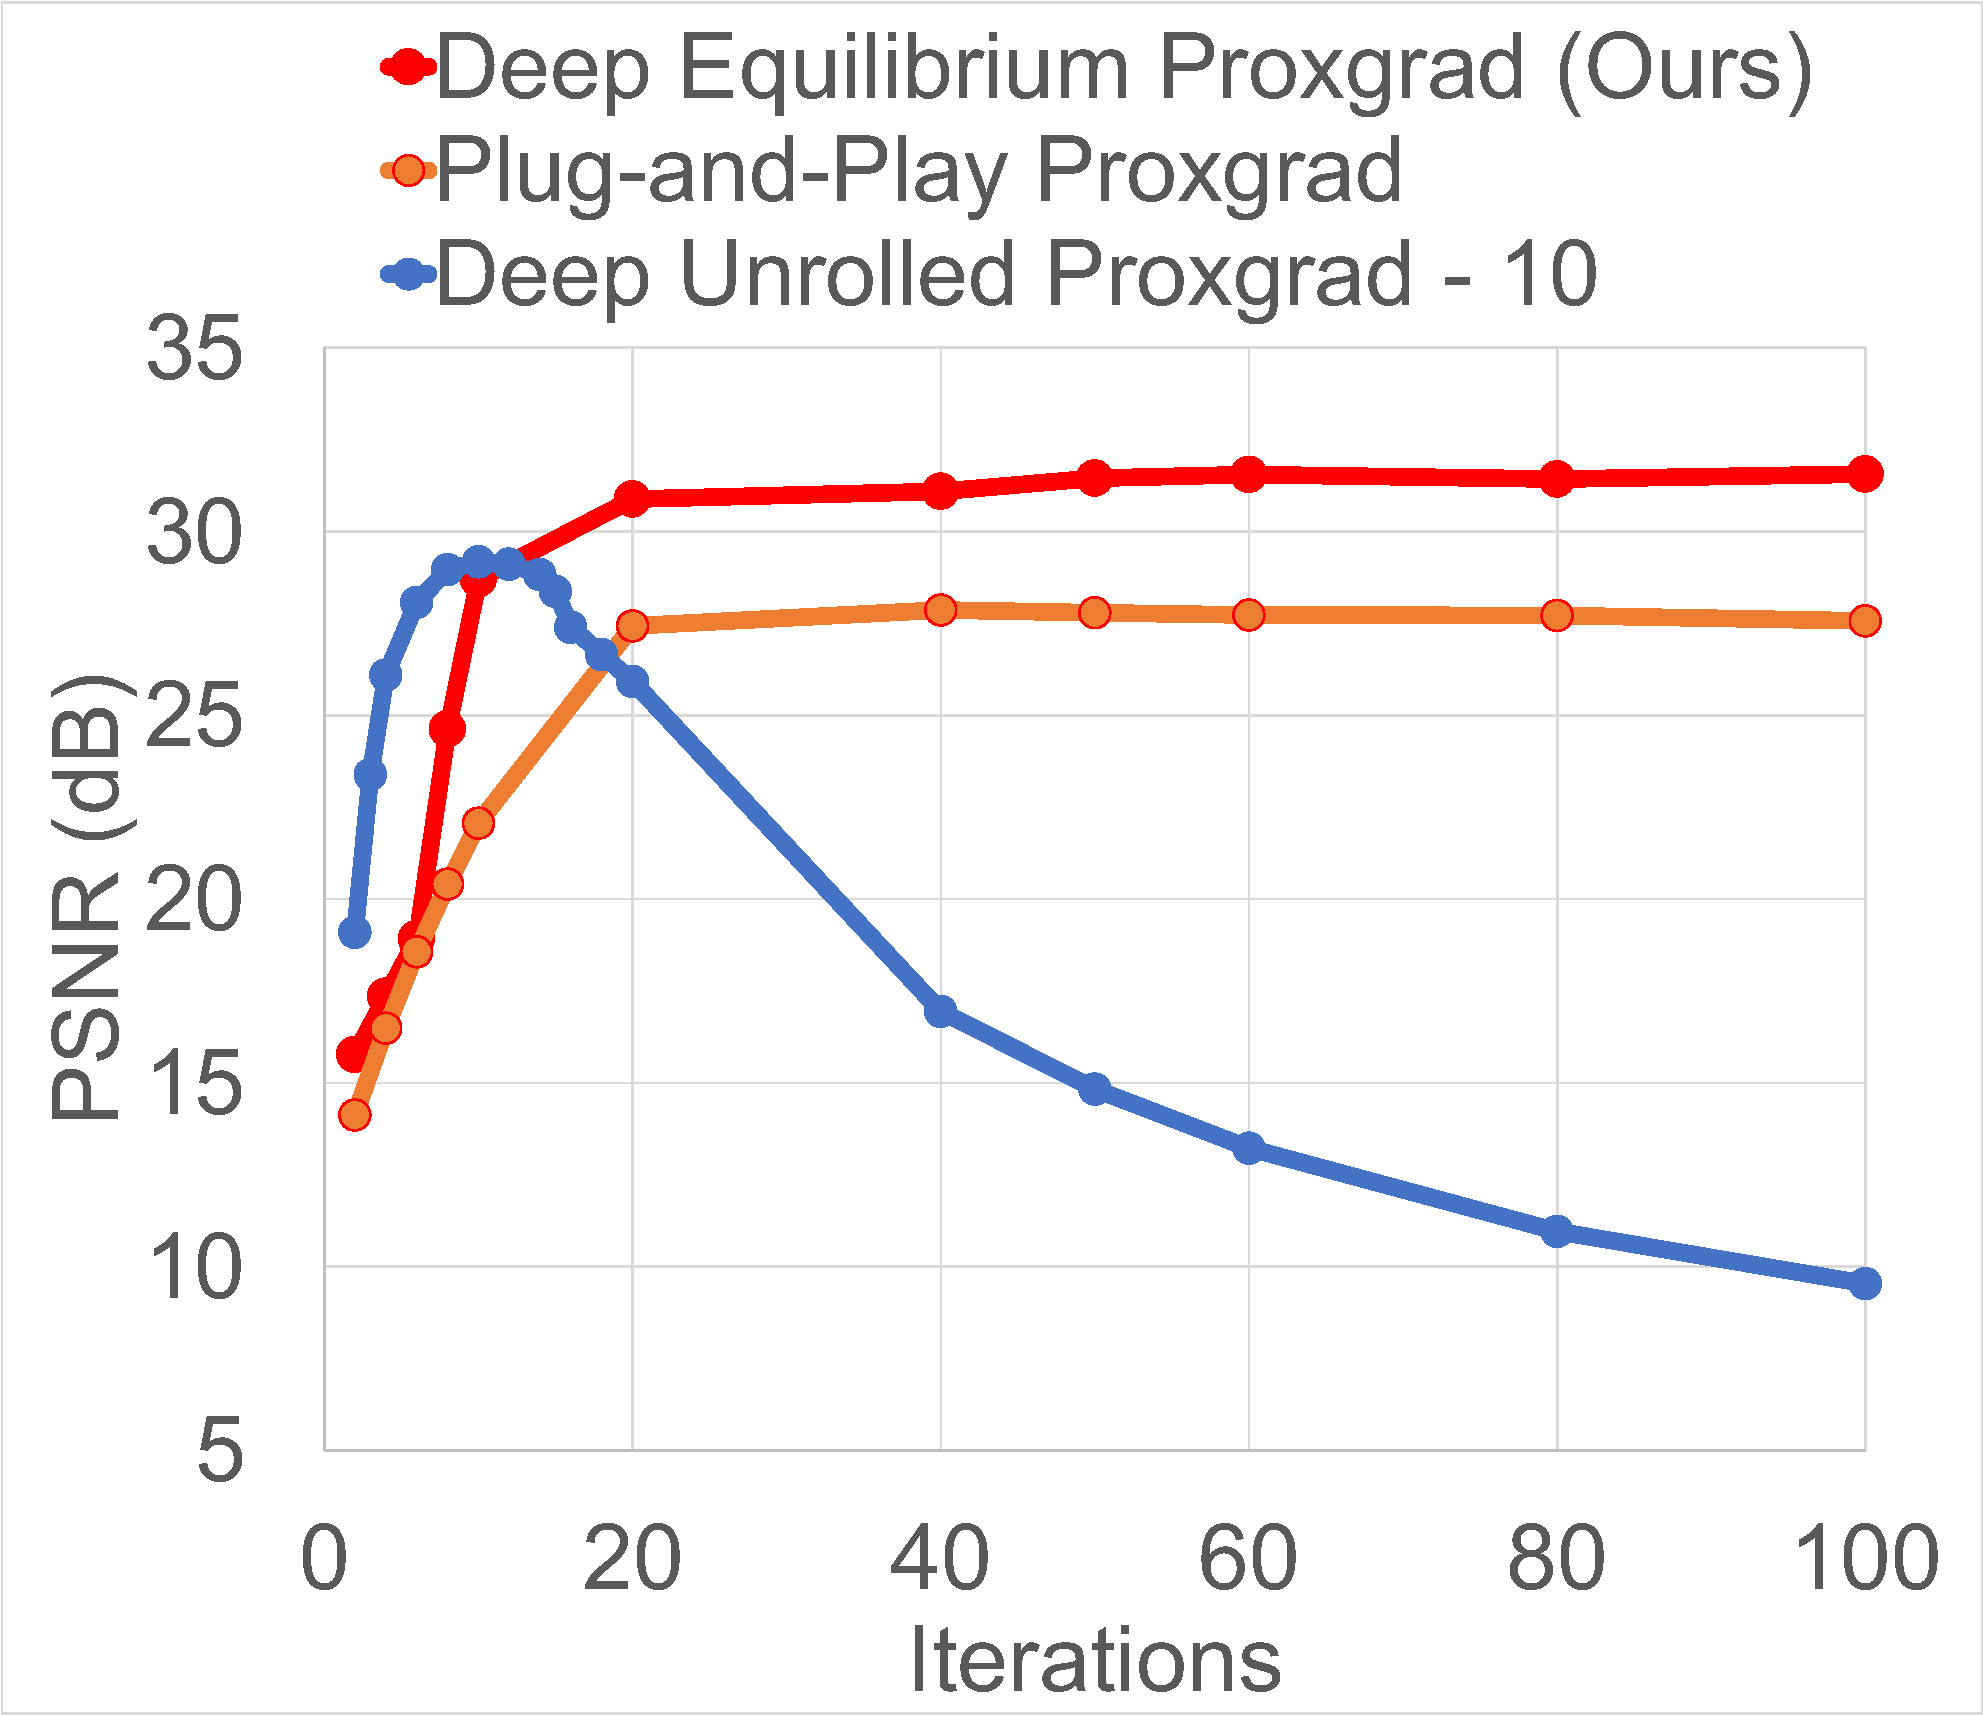
\includegraphics[width=\textwidth]{../Common_Images/deq/ResultsCS.pdf}
            \end{figure}
        \end{column}
        \begin{column}{0.5\textwidth}
            \textbf{The Practical Accuracy-Time Knob:}
            \vspace{1em}
            \begin{itemize}
                \item Deep unrolling (DU-Prox) is primarily effective only at the exact number of iterations it was trained for.
                \item DE methods maintain and strictly improve quality over a broader iteration range.
                \item At test time, one can stop early for speed, or continue solving for maximum fidelity without risking artefact degradation.
            \end{itemize}
        \end{column}
    \end{columns}
\end{frame}

\section{Theoretical Link: DEQs vs. Bilevel Learning}

\begin{frame}{Theoretical Link: DEQs vs. Bilevel Learning}
    An alternative paradigm for data-driven inverse problems is \textbf{bilevel learning}.
    
    \vspace{1em}
    The goal is to learn a regulariser such that the minimiser of the resulting variational problem closely matches the ground-truth data. This requires solving an upper-level risk minimisation problem constrained by a lower-level variational problem \cite{riccio2022regularization}.
\end{frame}

\begin{frame}{Recap: Bilevel Optimisation Formulation}
    Given training sets of ground-truth images $({\color{darkgreen}u_i^\dagger})$ and noisy measurements $({\color{uclred}f_i^\delta})$, bilevel learning seeks parameters $\Psi$ that yield
    
    $$ \min_\Psi \frac{1}{N} \sum_{i=1}^N \mathcal{L}(u_i^\star(\Psi), {\color{darkgreen}u_i^\dagger}) $$
    
    subject to the lower-level optimality condition
    
    $$ u_i^\star(\Psi) \in \arg\min_u \left\{ \frac{1}{2}\|{\color{uclblue}K}u - {\color{uclred}f_i^\delta}\|_2^2 + \mathcal{R}_\Psi(u) \right\} $$
\end{frame}

\begin{frame}{First-Order Optimality in Bilevel}
    When the parameterised regulariser $\mathcal{R}_\Psi$ is chosen such that the lower-level objective is strongly convex and differentiable, the unique minimiser $u^\star(\Psi)$ is fully characterised by the first-order optimality condition.
    
    \vspace{1em}
    This yields
    $$ {\color{uclblue}K^\top}({\color{uclblue}K} u^\star - {\color{uclred}f^\delta}) + \nabla \mathcal{R}_\Psi(u^\star) = 0 $$
\end{frame}

\begin{frame}{Bilevel Learning as a Restricted DEQ}
    Riccio et al. \cite{riccio2022regularization} observed that bilevel learning schemes are naturally a \textbf{subclass} of Deep Equilibrium Models!
    
    \vspace{1em}
    If we solve the lower-level problem via gradient descent, the optimal solution $u^\star$ inherently satisfies the fixed-point equation
    $$ u^\star = u^\star - \eta \left( {\color{uclblue}K^\top}({\color{uclblue}K} u^\star - {\color{uclred}f^\delta}) + \nabla \mathcal{R}_\Psi(u^\star) \right) $$
    
    \pause
    \vspace{1em}
    This is mathematically equivalent to learning the parameters $\Psi$ of a DEQ map defined by
    $$ f_\Psi(u; {\color{uclred}f^\delta}) := u - \eta \nabla \Phi(u, {\color{uclred}f^\delta}; \Psi) $$
\end{frame}

\begin{frame}{The Core Distinction: Potential vs. General Map}
    \begin{columns}
        \begin{column}{0.5\textwidth}
            \textbf{Bilevel Learning:}
            The map $f_\Psi$ is structurally constrained. It must be the update step of an optimisation algorithm minimising a potential function (representing a \emph{conservative vector field}).
        \end{column}
        \begin{column}{0.5\textwidth}
            \textbf{Deep Equilibrium Models:}
            Learn a purely general map $f_\theta$ that does \textbf{not} need to correspond to any energy minimisation process. 
        \end{column}
    \end{columns}
    
    \vspace{1em}
    
\end{frame}

\begin{frame}{Interpretability vs. Flexibility}
    Which framework should we choose?
    
    \vspace{1em}
    \begin{itemize}
        \item \textbf{Bilevel frameworks} offer incredibly strong \textbf{interpretability}, because the learned object is a mathematically rigorous regulariser existing within a clean variational energy formulation.
        \item \textbf{DEQs} offer greater \textbf{flexibility}. By removing the strict integrability constraint (that the update field must be a gradient), DEQs can learn vastly more effective fixed-point dynamics.
    \end{itemize}
\end{frame}

\begin{frame}{Visual Comparison: Inpainting Task}
    \begin{figure}[htpb]
        \centering
        \begin{minipage}{0.48\textwidth}
            \centering
            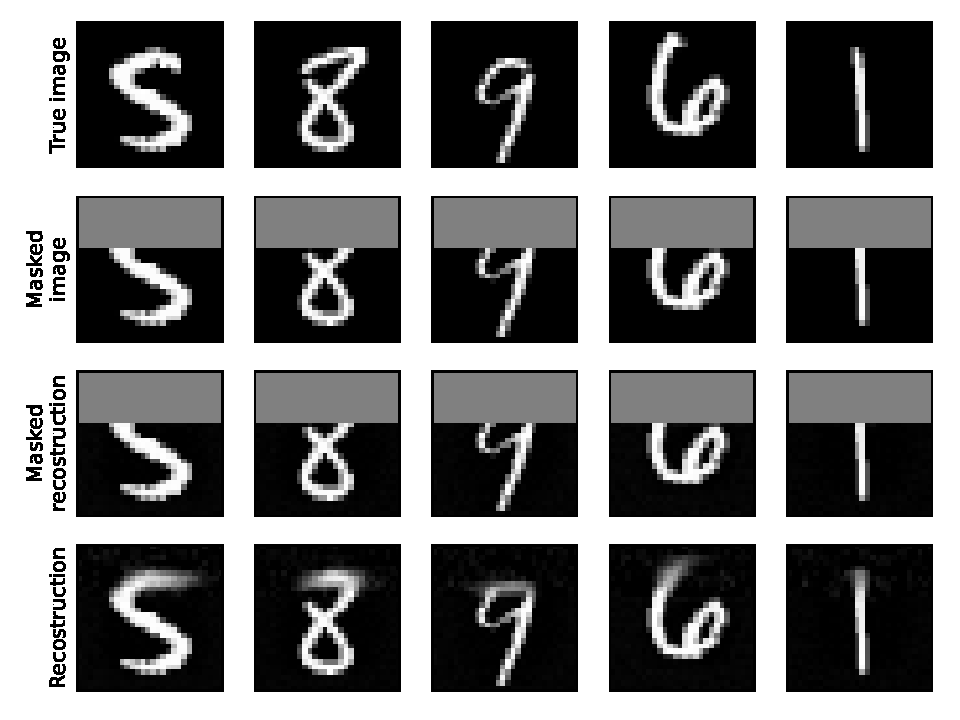
\includegraphics[width=0.9\textwidth]{../Common_Images/deq/riccio_inpainting_bl_test.pdf}
            \caption*{Bilevel Learning (BL)}
        \end{minipage}
        \hfill
        \begin{minipage}{0.48\textwidth}
            \centering
            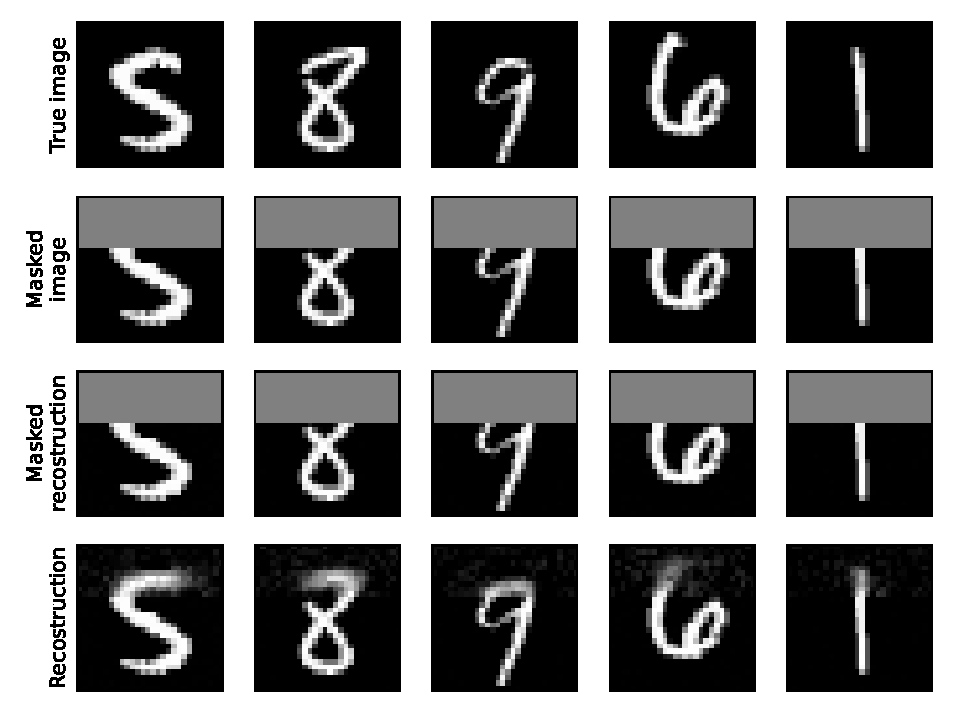
\includegraphics[width=0.9\textwidth]{../Common_Images/deq/riccio_inpainting_deq_test.pdf}
            \caption*{Deep Equilibrium (DEQ)}
        \end{minipage}
        \caption{Qualitative results for MNIST inpainting. Both the integrability-constrained bilevel framework and the unconstrained deep equilibrium method successfully reconstruct the image \cite{riccio2022regularization}.}
        \label{fig:riccio_visual_comparison}
    \end{figure}
\end{frame}

\begin{frame}{Empirical Robustness: DEQ vs. Bilevel}
    \begin{figure}[htpb]
        \centering
        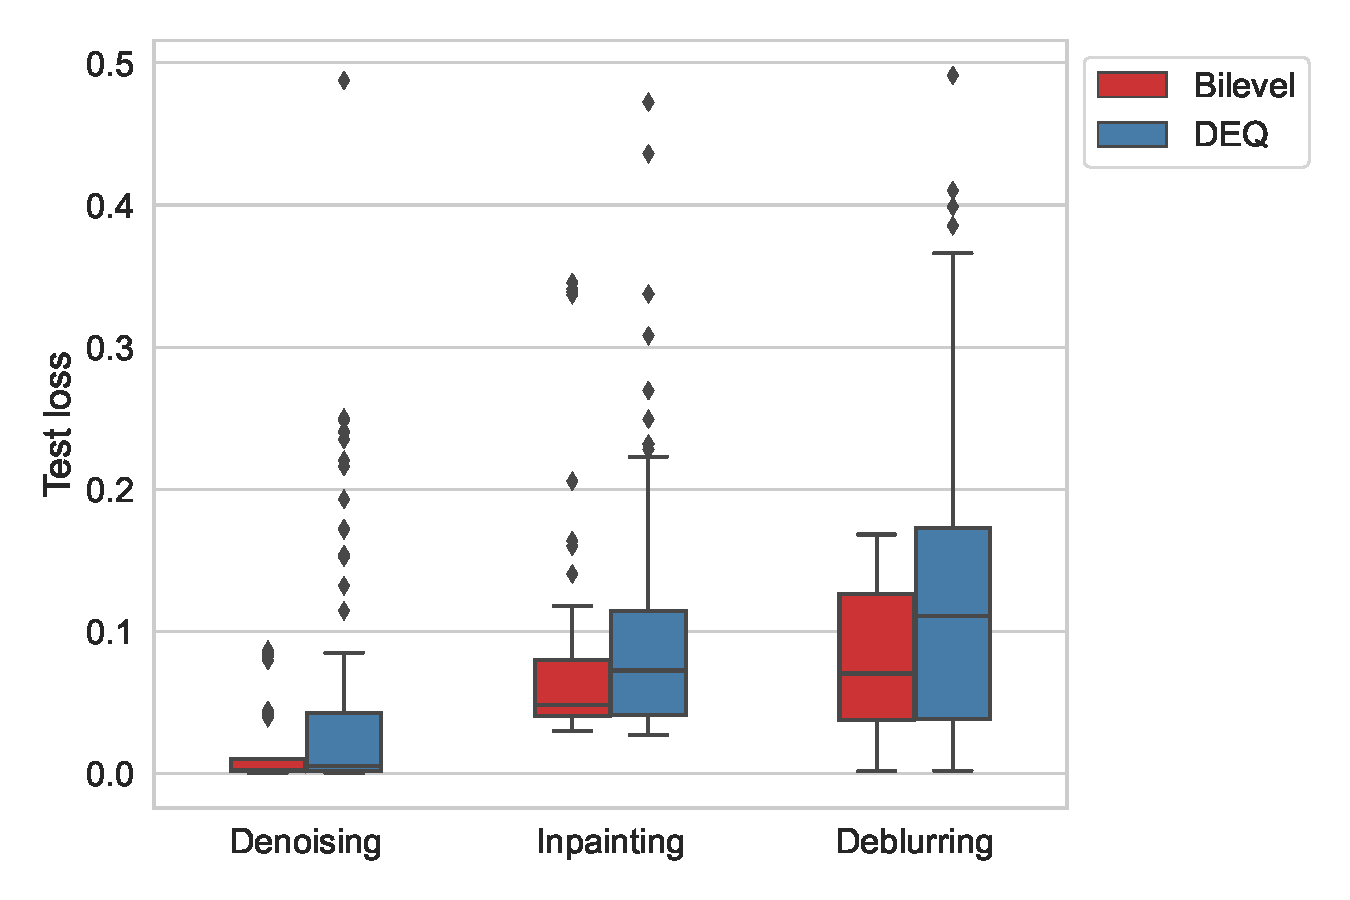
\includegraphics[width=0.5\textwidth]{../Common_Images/deq/boxplot_comparison_tasks.pdf}
        \caption{Boxplots illustrating the test dataset loss across various hyperparameter configurations. This demonstrates the general performance advantage of DEQs, but the structural robustness advantage of Bilevel learning \cite{riccio2022regularization}.}
        \label{fig:deq_vs_bl_boxplot}
    \end{figure}
\end{frame}

\begin{frame}{Summary of Lecture 3}
    \begin{itemize}
        \item \textbf{DEMs:} Deep Equilibrium Models for Imaging translate finite unrolled algorithms into robust, infinite-depth equilibrium models.
        \item \textbf{Avoiding Truncation:} They successfully bypass train-test unrolling truncation errors and provide critical adaptability at inference time.
        \item \textbf{Architectures:} We defined highly effective stable solvers including DE-GRAD, DE-PROX, and DE-ADMM.
        \item \textbf{Theoretical Connections:} Continuous bilevel learning is a structurally constrained, subclass of Deep Equilibrium Models.
    \end{itemize}
\end{frame}

\begin{frame}[allowframebreaks]{References}
    \bibliographystyle{abbrv}
    \bibliography{../../Lecture_Notes/references}
\end{frame}

\end{document}